\PassOptionsToPackage{top=3cm,left=3cm,right=3cm,bottom=3cm}{geometry}
\documentclass[fleqn,11pt]{wlscirep}

\usepackage{import}
\usepackage{main}

\renewcommand{\paragraph}[1]{\vspace{0.3cm}\noindent\underline{\emph{#1}}\hfill\noindent}

\begin{document}

\doublespacing

\title{\bfseries\LARGE\singlespacing{Molecular detection of SARS-CoV-2 and other respiratory viruses in saliva and classroom air: a two winters tale}}

% author list
\author[1,2]{Nicolas Banholzer}
\author[2,4]{Pascal Bittel}
\author[2,3]{Philipp Jent}
\author[4]{Lavinia Furrer}
\author[1]{Kathrin Zürcher}
%\author[1]{Simon Bertschinger}
%\author[5]{Ernest Weingartner}
%\author[2,4]{Alban Ramette}
\author[1,6,7]{Matthias Egger}
\author[2,8]{Tina Hascher}
\author[1*,2]{Lukas Fenner}

\affil[1]{Institute of Social and Preventive Medicine, University of Bern, Bern, Switzerland}
\affil[2]{Multidisciplinary Center for Infectious Diseases, University of Bern, Bern, Switzerland}
\affil[3]{Department of Infectious Diseases, Inselspital, Bern University Hospital, University of Bern, Bern, Switzerland}
\affil[4]{Institute for Infectious Diseases, University of Bern, Bern, Switzerland}
%\affil[5]{Institute for Sensors and Electronics, University of Applied Sciences and Arts Northwestern Switzerland, Windisch, Switzerland}
\affil[5]{Population Health Sciences, University of Bristol, Bristol, UK}
\affil[6]{Centre for Infectious Disease Epidemiology and Research, University of Cape Town, Cape Town, South Africa}
\affil[7]{Institute of Educational Science, University of Bern, Bern, Switzerland}

\affil[*]{Corresponding author: lukas.fenner@unibe.ch}


\vspace{2em}

%TC:ignore

\begin{information}\normalfont
\textbf{Word count:} Abstract 248 (max 250), Manuscript 1,230 (max 1,200) \\
\textbf{Display items:} Figure 1 (max 2) \\
\textbf{References:} 15 (max 15) \\
%\textbf{Supporting information:} STROBE checklist, Supplementary Data with texts, tables, and figures
% \par
\end{information}

\begin{abstract}\normalfont
\noindent \textbf{Objectives:} To compare the prevalence of SARS-CoV-2 and other respiratory viruses in saliva and bioaerosols between two winters and model the probability of virus detection in classroom air for different viruses.

\noindent \textbf{Methods:} We analyze saliva, air, and air cleaner filter samples from studies conducted in two  Swiss secondary schools (age 14-17 years) over seven weeks during the winters of 2021/22 and 2022/23. Two bioaerosol sampling devices and HEPA filters from air cleaners were used to collect airborne virus particles in five classrooms. Daily bioaerosol samples were pooled for each sampling device before PCR analysis of a panel of 19 respiratory viruses and viral subtypes. The probability of detection of airborne viruses was modelled using an adjusted Bayesian logistic regression model.

\noindent \textbf{Results:} Three classes (58 students) participated in 2021/22, and two classes (38 students) in 2022/23. During winter 2021/22, SARS-CoV-2 dominated in saliva (19 of 21 positive samples) and bioaerosols (9 of 10). One year later, there were 50 positive saliva samples, mostly influenza B, rhinovirus, and adenovirus, and two positive bioaerosol samples, one rhinovirus and one adenovirus. The probability of weekly airborne detection was 34\% (95\%-credible interval [CrI] 22\%$-$47\%) for SARS-CoV-2 and 10\% (95\%-CrI 5\%-16\%) for other respiratory viruses. 

\noindent \textbf{Conclusions:} There was a distinct shift in the distribution of respiratory viruses from SARS-CoV-2 during the Omicron wave to other respiratory viruses one year later. SARS-CoV-2 is more likely to be detected in the air than other endemic respiratory viruses, possibly reflecting viral characteristics that facilitate airborne long-range transmission.  \medskip

\par
\end{abstract}

\flushbottom
\maketitle

\vspace{2em}

\vspace{0.5em}

\noindent\textbf{Keywords:} respiratory viruses; SARS-CoV-2; influenza; airborne transmission; molecular detection
% maximum of 3-5 keywords

\thispagestyle{empty}
\sloppy
\raggedbottom

\newpage
%TC:endignore

\setcounter{page}{1}

\section*{Introduction}

The transmission of respiratory viruses, such as SARS-CoV-2 and influenza, in schools and other indoor environments is difficult to control\cite{Leung2020NatMed}. During the COVID-19 pandemic, non-pharmaceutical interventions and physical distancing reduced the spread of SARS-CoV-2 and other seasonal respiratory viruses, but a resurgence of respiratory infections followed the relaxation of these measures\cite{Poole2020LancetRespMed,Sauteur2022EuroSurv,Kandeel2023BMC}. Following epidemic peaks, a shift in the circulation of respiratory viruses occurs\cite{Pierangeli2012CMI}, which can be identified by frequent collection of non-invasive saliva samples\cite{Pasomsub2021CMI}. 

Respiratory viruses spread via multiple routes, including respiratory particles such as large droplets and small aerosols. Unlike larger droplets, which settle quickly, aerosols can remain suspended in the air for extended periods\cite{Wang2021}. Airborne infectious pathogens are primarily found in smaller particles and the distribution is similar across various pathogens\cite{Fennelly2020}. Thus, pathogen-carrying aerosols have the potential for long-range transmission, but the larger concentration of particles near the infectious person favors short-range transmission\cite{Wang2020}. 

%The complexity of airborne transmission lies in the interplay between the physicochemical properties of pathogen-carrying aerosols and environmental conditions\cite{Wang2021}, making it challenging to devise effective public health strategies to mitigate the spread of respiratory infections in various indoor settings, including schools, offices, and hospitals.

We compared saliva samples, bioaerosol samples, and samples from the HEPA-filters of air cleaners that were collected as part of two studies conducted in a Swiss school setting in winter 2021/22 (during the SARS-CoV-2 omicron wave)\cite{Banholzer2023PLoSMed} and winter 2022/23\cite{Banholzer2023medRxiv}. 


\section*{Methods}

Data were collected in two secondary schools (students age 14-17~years) in the canton of Solothurn, Switzerland, during a seven-week study period from the end of January to the beginning of March. Three classes (two classrooms) participated in 2021/22 and two classes (two classrooms) in 2022/23. An air quality device (AQ Guard, Palas GmbH, Karlsruhe, Germany) continuously measured indoor CO$_2$ levels, temperature, and humidity. A detailed comparison of the study settings can be found in \supp~Table~\zref{tab:comp_study}. 

Testing for a panel of respiratory infections was performed weekly in 2021/22 and bi-weekly in 2022/23. Airborne respiratory viruses were collected in each classroom with a cyclonic bioaerosol sampling device (Coriolis Micro Air, Bertin Instruments Montigny-le-Bretonneux, France) and the BioSpot-VIVAS condensation particle growth collection device (Aerosol Devices Inc., Ft. Collins, CO, USA)\cite{Lednicky2016AST}. The HEPA filters from the portable air cleaner (Xiaomi Mi Air Pro 70m2, Shenzhen, China) were removed and divided into 20~fields. For each field, one swab moistened with sterile Phosphate-Buffered Saline was collected, amounting to a total of 20~swabs per filter. Saliva and airborne samples were transported to the laboratory and stored at $-$80°C until further processing\cite{Huber2021}. Before real-time (RT)-PCR analysis, daily bioaerosol samples were pooled for each sampling device and enriched using Amicon Ultra-15 Centrifugal filters as described previously\cite{Banholzer2023PLoSMed}. Saliva samples were analyzed directly without prior filtration/enrichment. The Allplex RV Master Assay (Seegene, Seoul, South Korea) detects a panel of 19 major respiratory viruses and viral subtypes, including SARS-CoV-2, influenza A/B virus, respiratory syncytial virus, metapneumovirus, adenovirus, rhinovirus, and parainfluenza virus. 

We used descriptive statistics to present differences in the type and number of respiratory viruses detected in saliva and airborne samples between 2021/22 and 2022/23. A Bayesian logistic regression model was used to estimate the probability of detecting any SARS-CoV-2 versus non-SARS-CoV-2 viruses in the air during a study week, adjusting for differences in the study settings and the interventions implemented during the studies (see \supp~Text~\zref{sec:model} for a detailed model description).   

\section*{Results}

In 2021/22, 58~students participated in weekly saliva testing. There were 21~positive saliva samples during the study, 19~SARS-CoV-2, one~influenza~A virus, and one~adenovirus (\Cref{fig:comparison}a, left). There were 10~positive bioaerosol samples, nine~SARS-CoV-2 and one~adenovirus. There were eight~positive samples on the HEPA-filters, six~SARS-CoV-2, one~influenza~A virus and one~adenovirus. In 2022/23, 38~students participated in bi-weekly saliva testing. There were 50~positive saliva samples, mostly influenza~B virus, rhinovirus, and adenovirus (\Cref{fig:comparison}a, right). There were two~positive bioaerosol samples, one~rhinovirus and one~adenovirus. There were four~positive samples on the HEPA-filters of the air cleaners, one~influenza~B virus, one~rhinovirus, one~adenovirus, and one~SARS-CoV-2. We found six positive air-saliva samples in the same week (4~SARS-CoV-2 and two~non-SARS-CoV-2 viruses (\Cref{fig:comparison}b), suggesting they were paired samples. 

SARS-CoV-2 was more likely detected in bioaerosols than other respiratory viruses (adjusted odds ratio 4.8, 95\%-CrI 2.6$-$9.0). The probability of airborne molecular detection was 34\% (95\%-credible interval [CrI] 22\%$-$47\%) for SARS-CoV-2 versus 10\% (95\%-CrI 5\%-16\%) for non-SARS-CoV-2 viruses (\Cref{fig:comparison}c). We adjusted estimates for differences in maximum daily CO$_2$, which increased from 1,134\,ppm (standard deviation [SD] 277\,ppm) in 2021/22 to 2,224\,ppm (SD 321\,ppm) in 2022/23. Relative humidity and temperature were similar at around 38\% and 20°C, respectively. 

\begin{figure}
    \centering
    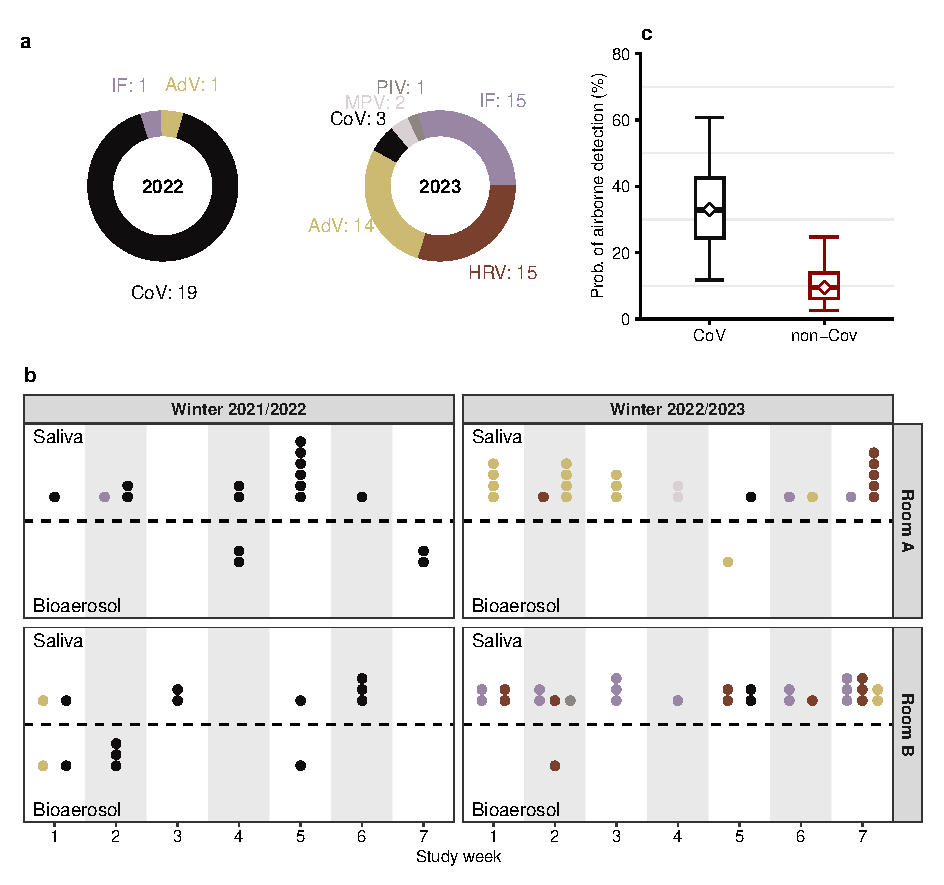
\includegraphics{results/comparison.pdf}
    \caption{Comparison of molecular detection of respiratory viruses between winter 2021/22 and winter 2022/23. \textbf{(a)}~Distribution of respiratory viruses found in saliva. IF: influenza~A/B virus, HRV: human rhinovirus, AdV: adenovirus, CoV: SARS-CoV-2, MPV: human metapneumovirus, PIV: parainfluenza virus. \textbf{(b)}~Positive samples in saliva and bioaerosols per study week. \textbf{(c)}~Probability of detecting any SARS-CoV-2 and non-SARS-CoV-2 viruses in bioaerosols during a study week (posterior mean as dots, interquartile range as box, 95\%-CrI as error bars).}
    \label{fig:comparison}
\end{figure}


\section*{Discussion}

% In comparison, 

We compared the molecular detection of respiratory viruses in saliva, air, and filter samples collected in two studies in Swiss secondary schools in the winter seasons of 2021/22 and 2022/23. In winter 2021/22, we predominantly identified SARS-CoV-2 in saliva, air, and air filter samples. Conversely, in 2022/23, we primarily detected non-SARS-CoV-2 viruses, such as influenza viruses and adenoviruses, in saliva samples, but these were rarely found in air or filter samples. 

Overall, the likelihood of molecular airborne detection was substantially higher for SARS-CoV-2 compared to non-SARS-CoV-2 viruses, even when we adjusted for covariates and differences between the studies. Besides differences in virus circulation in the population during the study periods, a plausible explanation is that SARS-CoV-2 can remain airborne for extended durations, thus facilitating long-range transmission, matching the observation of superspreading events during the pandemic. This is in contrast to other respiratory viruses, where airborne detection was found to be infrequent in our studies. Therefore, prolonged close contact may be relatively more important for transmission of respiratory viruses other than SARS-CoV-2, although close contact also facilitates transmission of SARS-CoV-2\cite{Leung2020NatMed,Lind2023NatCommun}.

Technical factors are unlikely to account for the differences in airborne detection. The two studies employed identical bioaerosol samplers and laboratory methods, and no technical problems occurred. Temperature and relative humidity were also similar. Ventilation changed, with higher CO$_2$ levels in 2022/23 potentially enhancing airborne survival, but this and other differences were controlled for in the statistical analysis. Therefore, it is plausible that the difference in airborne detection may be due to differences in virus characteristics, particularly between SARS-CoV-2 and non-SARS-CoV-2 viruses, which may influence the generation and survival of airborne viral RNA\cite{Wang2021}. Non-SARS-CoV-2 respiratory virus infections may results in smaller amounts of exhaled bioaerosols, falling below the detection limit of current sampling devices\cite{Belser2023PLOSPath}. 

In conclusion, we observed a distinct shift in the distribution of respiratory viruses from SARS-CoV-2 in the winter of 2021/22 to non-SARS-CoV-2 viruses in 2022/23, reflecting the transition from epidemic to endemic transmission of SARS-CoV-2. Molecular detection of airborne SARS-CoV-2 was more frequent than other endemic respiratory viruses. Future studies should investigate the seasonality of SARS-CoV-2 and non-SARS-CoV-2 respiratory viruses and the contribution of close contact versues airborne long-range transmission to overall transmission of respiratory infections in congregate indoor settings.   


\bibliography{references.bib}

\end{document}